% TODO:
% Why are we focusing on Spark Streaming?
%
To understand our work, we provide a short description of Spark Streaming's architecture.
\begin{figure}[t!]
  \begin{center}
    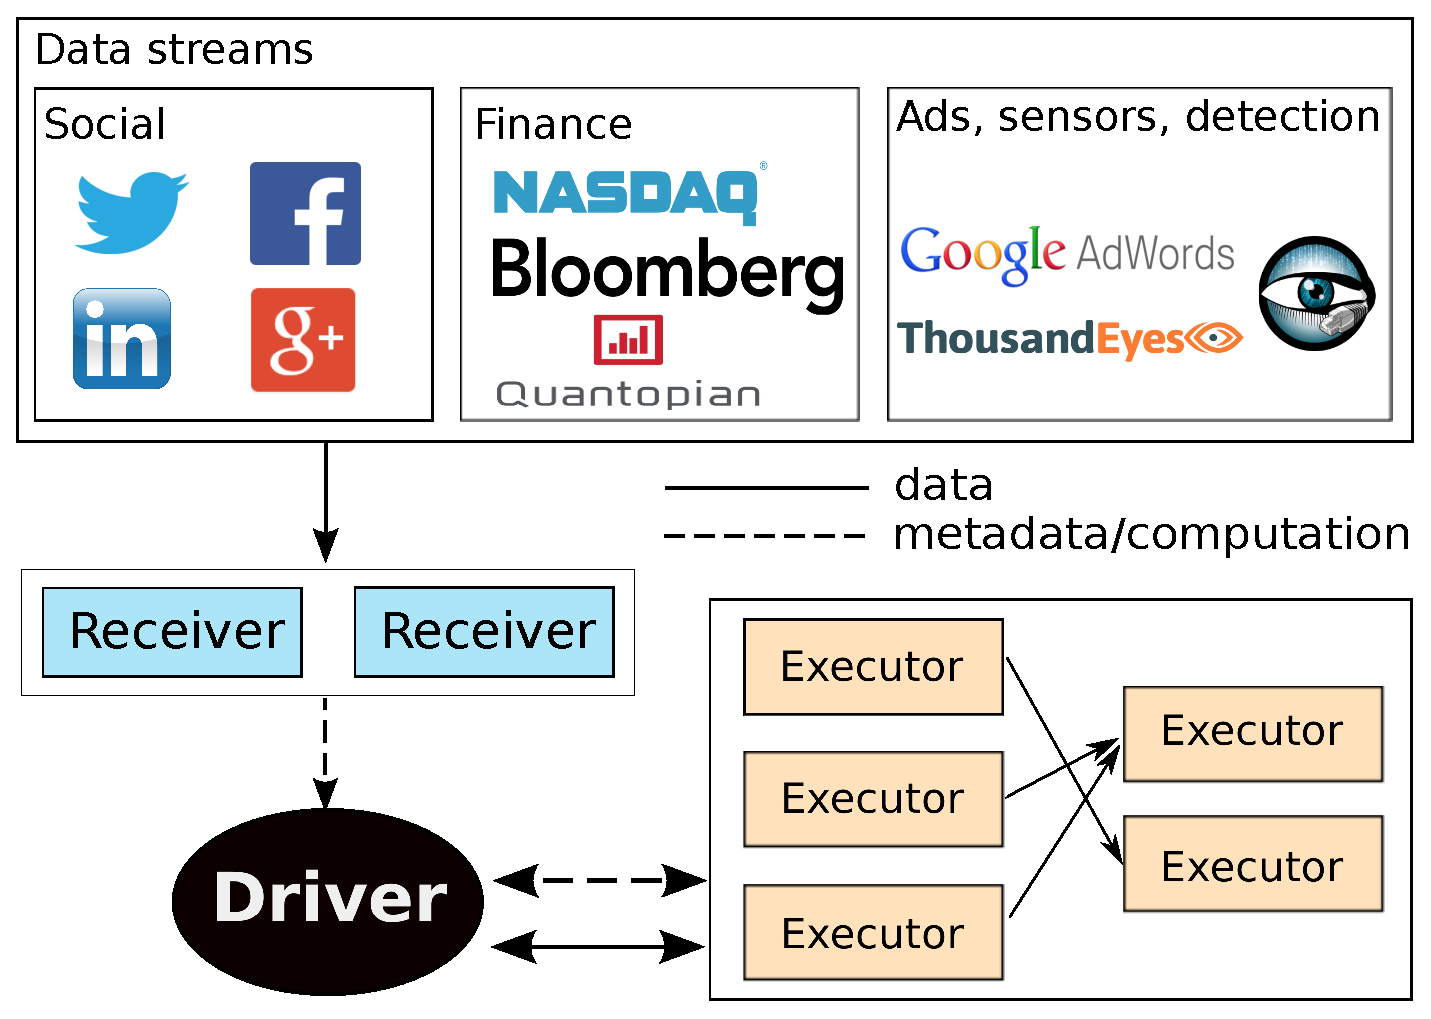
\includegraphics[scale=0.35]{images_graphs/spark_architecture_v4.eps}
  \end{center}
  \caption{Diagram of a Spark Streaming work flow. A Receiver and an Executor may execute in the same node.}
  \label{fig:SparkStreaming_architecture}
\end{figure}

Spark~\cite{Spark} is a general-purpose engine for large-scale cluster computing. It operates on Resilient Distributed Datasets (RDDs), an abstraction that represents read-only collections of objects partitioned across a set of machines. RDDs can be created from raw data or other RDDs. 
RDDs keep track of the bulk operations (e.g., map and reduce) performed on data (lineage) so that partitions can be recomputed if they are lost due to failures. 
Another feature of RDDs is that they can be persisted in memory, allowing efficient iterative computations.

Spark Streaming, the focus of our work, is a stream processing engine built on top of Spark.
It implements an abstraction called discretized streams (D-Streams), which takes advantage of RDDs to provide computations over windows of streaming records.
%which take advantage of RDDs to provide fast recovery after failures. 
The abstraction allows a micro-batch approach to streaming data, yielding high throughput, scalability and fault-tolerance.


The execution of a Spark Streaming job works as depicted in Figure~\ref{fig:SparkStreaming_architecture}. 
First, data is generated at a source (e.g., tweets from Twitter). As the data is generated, it is pushed to Spark Streaming, and is received by a Receiver. 
The Receiver is responsible for receiving input data and stash it in memory. Periodically, every \texttt{blockInterval} milliseconds, the Receiver takes the data stashed in memory and generates a block with it.
Once a block is generated, the Receiver informs a Spark Streaming's central component called Driver about this block. The Driver is responsible for holding metadata about the records received. 
Periodically, every \texttt{batchInterval} milliseconds, the Driver takes the blocks that have been communicated by the receivers and that have not been processed yet and generates a batch job. 
Once this batch job is generated it is appended to a queue of jobs to be scheduled. 
The scheduler continuously polls this queue and schedules the jobs in the machines available in the cluster.
Jobs are run in stateless isolated environments called Executors. Executors are usually deployed in the same nodes as Receivers.
Every batch job is divided into map and reduce stages, each of which contains tasks that need to be scheduled.

At the heart of the micro-batches approach taken by Spark is a trade-off between the amount of records Spark can process per unit of time and the time the system takes to return to the user the result of processing a stream record.
On one hand, waiting for more records to generate bigger batches allows Spark Streaming to amortize its overheads. On the other hand, the more time the system waits for data, the less responsive the system is.
Moreover, Spark can provide window semantics over data. For instance, a user can easily use Spark Streaming to compute the average temperature during the last 30 minutes over a stream of temperature sensor data.
%    This means that users can ask the system to compute 

%Internally, a variable called block interval controls the period of time before a receiver generates a new block. The total number of blocks generated in a batch interval corresponds to the number of tasks spawned for every stage of the resulting batch job.

Internally, Spark Streaming makes extensive use of Actors -- a design pattern that decouples the invocation of methods from their execution. 
In this approach, the invocation of methods between certain components is performed by inserting a message in a queue of the message receiver.
The component that receives the message continuously polls the queue and services messages in parallel.
This approach has been shown to provide high levels of concurrency and adaptability to changing loads~\cite{SEDA}.
